\newpage
\part{Platforma Gisquick}
\newpage

\section{Úvod do Gisquick}

Gisquick je webová mapová publikační platforma s otevřenými daty. Jejím
účelem je snadné a rychlé publikování projektů vytvořených v programu
QGIS, které je možné posléze prohlížet na webovém rozhraní platformy
Quisqick.
Celá platforma se skládá z několika komponentů (jejich obecné fungování
je popsáno v kapitole \ref{sssec:fungovani-platforem} ). Komponenty jsou
následující.

\subsection{Komponenty}
\label{sssec:gisquick-komponenty}


\begin{itemize}
\item\textit{Gisquick plugin} - jedná se o zásuvný modul pro
program QGIS, pomocí kterého je možné existující projekt
publikovat. Publikace je nutná pro pozdější použití projektu
na platformě Gisquick. Během samotné publikace si může každý
uživatel projekt nastavit tak, aby zobrazovaný předmět zájmu
přesně odpovídal jeho požadavkům (možnost selekce jednotlivých
vrstev, nastavení maximálního a minimálního měřítka,
atd.). Gisquick plugin pracuje zcela odděleně od ostatních
komponentů a jeho výstupem je složka obsahující všechny použité
vrstvy, uložený projekt ve formátu .qgs a metadatový soubor. Ten
obsahuje nastavení provedené během procesu publikace a dále popis
projektu. Metadatový soubor je použit pro potřeby webového klienta.
\item\textit{webový server} - webový server zpracovává
dotazy z webového klienta ve formě OGC standardů (viz. kapitola
\ref{sssec:ogc}). Následně odpovídá například ve formě mapových
obrazů. Na straně webového serveru je použit aplikační rámec Django,
který je stejně jako Gisquick plugin psaný v jazyce Python.
\item\textit{QGIS server} - jedná se o webový mapový server
na základě kterého jsou vytvářeny mapové obrazy. Použití
QGIS serveru je dáno skutečností, že veškeré mapové prvky
zde vytvořené korespondují svým vzhledem s prvky vytvořenými
v QGIS desktopové aplikaci. Díky tomu si může být uživatel
jistý tím, že publikovaný projekt bude věrně odpovídat jeho
původnímu projektu.
\item\textit{webový a mobilní klient} - klient uživateli nabízí
uživatelské rozhraní celé aplikace, ve kterém se může
orientovat a pomocí kterého interaguje s webovým serverem a tak
mění zobrazovaný obsah. Právě této části spolu s Gisquick
pluginem byla je v této práci věnována největší pozornost.
\end{itemize}

\subsection{Uživatelské rozhraní}

\begin{figure}[h!]
\centering
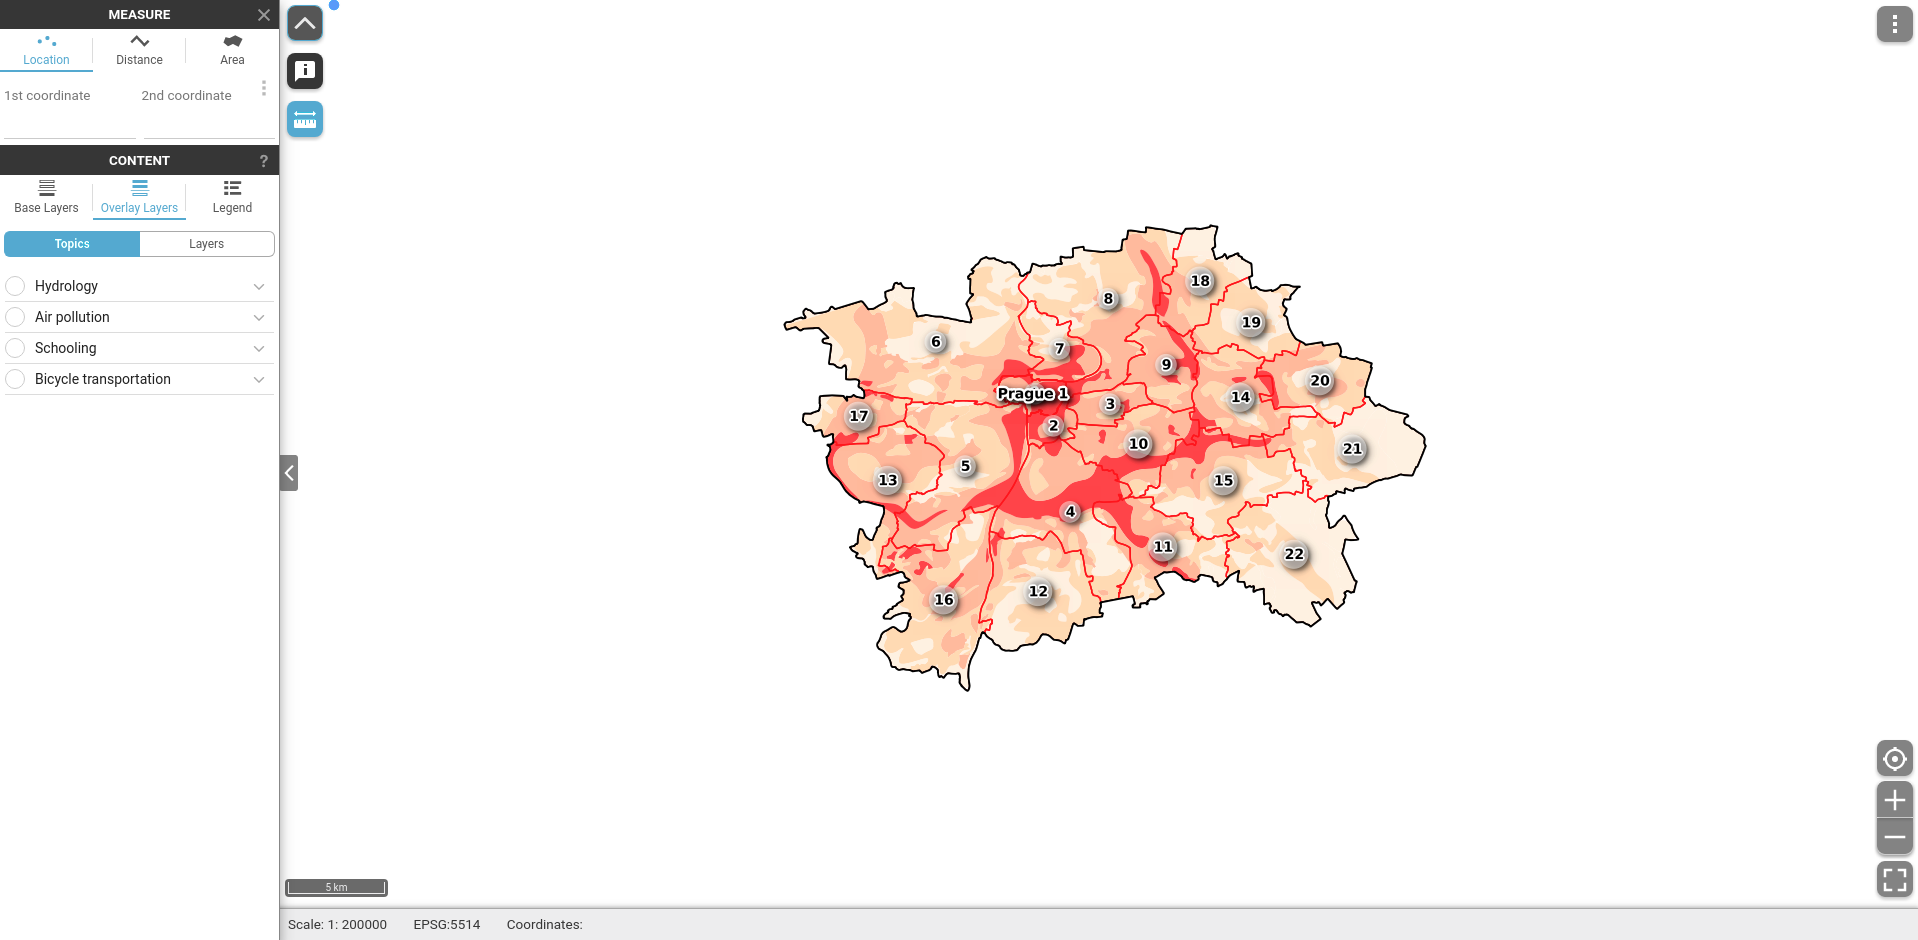
\includegraphics[width=0.9\textwidth]{../img/gisquick_ui.png}
\caption{Ukázka uživatelského rozhraní platformy
Gisquick\cite{gisquick-prague}}
\label{fig:gisquick-prague}
\end{figure}

Obrázek výše zachycuje webové uživatelské rozhraní platformy
Gisquick. Jedná se o sadu velice jednoduchých a intuitivních nástrojů
sloužících pro snadnou orientaci v publikovaném projektu, filtraci
jednotlivých částí a provádění jednoduchých operací. Například
měření vzdáleností na mapě.

Uživatel má být schopný rychlé a intuitivní orientace jak v projektu,
tak v samotné webové aplikaci. K tomu slouží postranní menu se správou
vrstev spolu s menu nástrojů, které je v obrázku \ref{fig:gisquick-prague}
rozbaleno. V horní postranního menu části je právě aktivovaný
nástroj sloužící k zjišťování souřadnic, měření vzdáleností
a ploch. Hlavní část je věnována interaktivní mapové kompozici. Ta
poskytuje možnost změny velikosti a polohy výřezu zobrazovaného území.

\begin{figure}[h!]
\centering
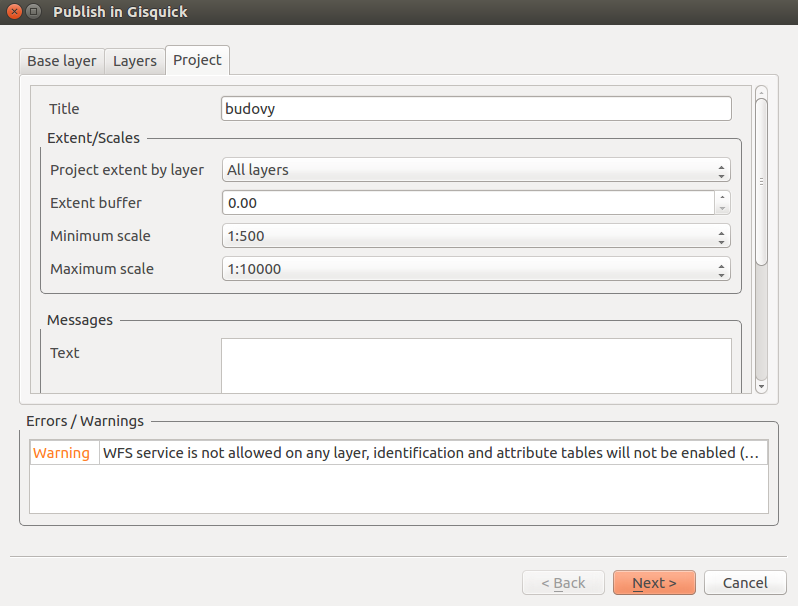
\includegraphics[width=0.7\textwidth]{../img/gisquick_plugin.png}
\caption{Ukázka uživatelského rozhraní Gisquick pluginu pro QGIS}
\label{fig:gisquick-plugin}
\end{figure}

\newpage
Gisquick plugin pro QGIS rovněž disponuje uživatelským rozhraním, kde
pomocí jednoduchého dialogového okna jsou nabízeny možnosti nastavení
pro export vrstev. Jeho první část je rozdělena na tři záložky a
stavovou řádku, ve které se jsou vypisována chybová hlášení. V
první záložce \textit{Base layer} je možno nastavit podkladové vrstvy
jako například Open Street Map, nebo Binq mapy. V další záložce
\textit{Layers} je možno nastavit které vrstvy budou publikované. Při
implementaci podpory pro časoprostorová data bylo nastavení v této
záložce rozšířeny o další možnosti. Tomuto rozšíření se bude
práce věnovat detailněji v dalších částech. V poslední záložce je
obecné nastavení projektu. Další okno slouží k nastavení \textit{topics}
nebo-li tématicky orientovaných vrstev \cite{gisquick-manual}. Předposlední
stránka obsahuje pouze souhrn publikovaného projektu. Poslední zobrazuje
výpis souborů, které se po zmáčknutí tlačítka \textit{Publish}
vytvoří. Ty je posléze nutné nahrát na Gisquick publikační server.

\newpage
\subsection{Použité technologie}

\begin{figure}[h!]
\centering

\includegraphics[width=0.8\textwidth]{../img/technologies.png}
\caption{Loga níže popsaných softwarů}
\label{fig:technoogies}
\end{figure}

\noindent
\textbf{Vue.js} - jedná se o moderní aplikační rámec s otevřeným kódem
napsaný v programovacím jazyce JavaScript, jehož první verze byla vydaná
začátkem roku 2014 Evanem You \cite{vue-history}. Jeho hlavní použití je
vývoj uživatelského rozhraní aplikací, tedy na straně webového klienta
(viz. kapitola \ref{sssec:fungovani-platforem}). Uživatelské rozhraní
je za pomoci Vue.js rozděleno na několik  komponent, kdy každá obsahuje
vlastní JavaScript, HTML a CSS skripty. Jednotlivé komponenty dělají kód
přehlednější a aplikace výkonově méně náročnější. Protože vždy
jsou použity jenom ty komponenty, které koncový uživatel v danou chvíli
potřebuje. Mezi další výhody Vue.js patří mimo práce s komponenty
jeho reaktivita, a úpravu objektového modulu dokumentu (DOM).

Původní verze webového klienta Gisquicku jsou psány za použití
aplikačního rámce AngularJS. V současné chvíli je však celý klient
vytvářen znovu za pomoci Vue.js. Z toho důvodu bylo rozšíření platformy
o podporu časoprostorových dat na straně klienta psáno právě ve Vue.js.

\newpage
\bigskip
\noindent
\textbf{PyQt} - PyQt je vazba pro programovací jazyk Python, která umožňuje
využití aplikačního rámce pro Qt aplikace. Vazby jsou vytvořeny ve formě
Python modulů a obsahují okolo jednoho tisíce tříd. Jedná se o kombinaci
výhod nabízející jednoduchost Pythonu a obrovské schopnosti Qt v jednom
celku. Díky tomu je možné jednoduše vytvářet grafické uživatelské
rozhraní přímo za pomocí Pythonu. PyQt je software s otevřeným kódem,
který byl vytvořen britskou firmou Riverbank Computing a je nabízen pod
dvojí licencí GNU GPL v3 a komerční licencí společnosti Riverbank
\cite{pyqt}.

\bigskip
\noindent
\textbf{Docker} - Docker je počítačový program s otevřeným
kódem umožňující zapouzdření (izolaci) jednotlivých aplikací do
kontejnerů. Vytvořený kontejner se nazývá \textit{Docker image}. Obecné
pravidlo je použití pouze jedné aplikace pro jeden Docker kontejner. Docker
image mohou být posléze spuštěny na jakémkoli hardwaru s operačním
systémem Linux, nebo Windows, na který je Docker program nainstalovaný. Tato
skutečnost má obrovskou výhodu pro nasazení aplikací do produkčních
serverů, jejich sdílení s dalšími uživateli, nebo vytváření
clusterů složených z dílčích aplikací. Po spuštění aplikace v
Docker kontejneru není vytvořen nový virtuální stroj, ale aplikace
v kontejnerech využívají hostující operační systém. Výhod tohoto
řešení spočívá v minimalizaci velikosti kontejneru.

Gisquick pro své komponenty (mimo Gisquick pluginu) v produkční
verzi využívá právě použití Docker kontejnerů. Tímto způsobem
je možné celou Gisquick platformu jednoduše spustit na lokálních
zařízeních. Vývoj je tak jednodušší, protože odpadá jakékoli
nastavování vývojového prostředí.

\bigskip
\noindent
\textbf{OpenLayers} - jedná se o knihovnu napsanou v programovacím
jazyce JavaScript, která umožňuje správu a vizualizaci map ve webových
prohlížečích. Jedná se o software s otevřeným kódem nabízející
široké rozhraní pro tvorbu geografických aplikací. OpenLayers byly
vytvořeny soukromou společností MetaCarta v roce 2005. Od roku 2007
spadají OpenLayers pod organizaci OSGeo.

\newpage
\section{Implementace nástroje pro Gisquick plugin}

V kapitole \ref{sssec:gisquick-komponenty} jsou zmíněny výstupy z Gisquick
pluginu. Jedná se o složku obsahující projekt ve formátu .qgs, data
použita v projektu a metadatový textový soubor. Hlavním cílem úprav
Gisquick pluginu bylo vytvoření jednoduchého uživatelského rozhraní,
které umožňuje definovat všechny potřebné parametry sloužící ve
webovém klientu k inicializaci nástroje pro práci s časovými daty. Tyto
parametry jsou během publikace pro jednotlivé vrstvy nastavené a dále
vepsané do metadatového souboru.

\subsection{Uživatelské rozhraní}
\label{sssec:plugin-ui}

\begin{figure}[h!]
\centering
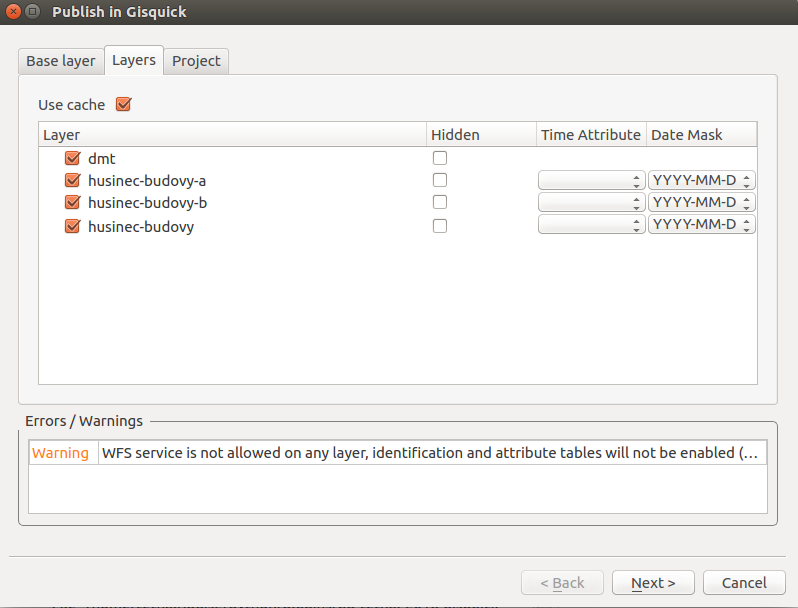
\includegraphics[width=0.9\textwidth]{../img/gisquick-plugin.png}
\caption{Nastavení vrstev v Gisquick pluginu}
\label{fig:gisquick-plugin-layers}
\end{figure}

Obrázek \ref{fig:gisquick-plugin-layers} zobrazuje dialogové okno publikace
projektu pomocí Gisquick pluginu. V prvním kroku publikace, v záložce
vrstvy \textit{Layers} je pro vektorové vrstvy přidáno nové nastavení. V
Případě rastrových, jako je například v obrázku zvolená vrstva dmt,
možnost nastavení časových vrstev není možná.

Ve sloupci \textit{Time Attribute} jsou v roletovém menu vypsány
všechny atributy každé vrstvy. Implicitní hodnota je prázdný textový
řetězec. Zde je nutné pro každou časovou vrstvu vybrat atribut, který
obsahuje časové hodnoty (dále jen časový atribut).

Sloupec \textit{Date Mask} obsahuje roletové menu s časovými formáty,
které určují jakým způsobem budou časová data na webovém klientu
zobrazena. Díky tomuto nastavení je možné, nehledě na formát časového
atributu, nastavit kterýkoli nabízený časový formát. V tomto formátu
budou zobrazeny časové hodnoty na webovém klientovy. V případě volby
formátu je nutné znát původní data. Přejde se tím situacím kdy
uživatel zvolí formát zobrazující pouze roky, zatímco původní data
budou v rozpětí jednoho dne.

Jestli jsou časové vrstvy dobře nastaveny, a výpočet proběhl korektně,
se lze v předposledním kroku publikace přesvědčit v souhrnu publikovaného
projektu (obrázek \ref{fig:publishing-summary}).

\begin{figure}[h!]
\centering
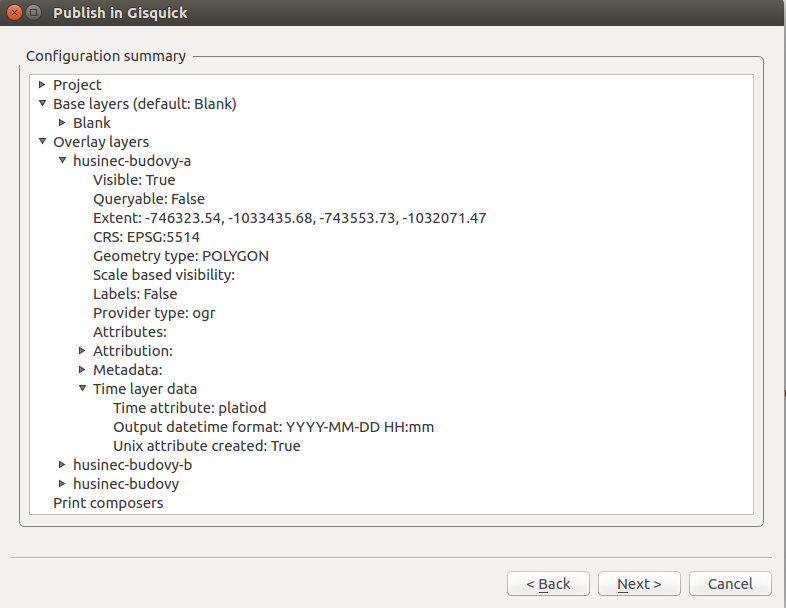
\includegraphics[width=0.9\textwidth]{../img/project-publishing-time-summary.png}
\caption{Souhrnu publikovaného projektu v Gisquick pluginu}
\label{fig:publishing-summary}
\end{figure}

\subsection{Funkcionalita}
\label{sssec:plugin-functionality}

Poté co uživatel v záložce \textit{Layers} nastaví všechny požadované
parametry může svou volbu potvrdit tlačítkem \textit{Next}, které
spustí výpočet a zobrazí další krok publikace.

Do výpočetního procesu se dostanou pouze ty vrstvy, které splňují dvě
podmínky. Jejich časový atribut musí existovat a nesmí být prázdným
textovým řetězcem. Tyto podmínky eliminují výpočet nad rastrovými
vrstvy. Dále zajistí to, že do výpočtu se dostanou pouze ty vrstvy,
které mají nastavený časový atribut. Tyto vrstvy jsou dále v textu
označovány jako časové.

Výpočet probíhá pro jednotlivé vrstvy splňující vstupní podmínky
totožně. Pro každou časovou vrstvu je volána metoda \verb|get_time_info|.

V prvním kroku metody \verb|get_time_info| je metodou
\verb|validate_time_attribute| vytvořena validační maska. Jedná se o pole,
které svou velikostí odpovídá počtu mapových prvků \textit{Features}
časové vrstvy. Každý prvek validační masky může nabývat různých
hodnot. Prvek může obsahovat časový formát textového řetězce, ve
kterém je časová hodnota uložena. Pokud však hodnota není v textovém
řetězci, nebo její časový formát textového řetězce neodpovídá
podporovaným formátům, je do daného prvku validační masky uložena
hodnota \textit{-1}. Podporované formáty jsou explicitně vypsány ve
zdrojovém kódu Gisquick pluginu v proměnné \verb|datetime_mask_array|.

Například pro časovou vrstvu obsahující šest prvků, kdy pouze pět
z nich má validní datum, a to ještě v odlišných časových formátech
může validační maska vypadat následovně:

\begin{verbatim}
[
'%Y-%m-%d',
'%Y-%m-%d',
-1,
'%Y-%m-%dT%H:%M:%S',
'%Y-%m-%dT%H:%M:%S',
'%Y-%m-%dT%H:%M:%S'
]
\end{verbatim}

Během vytváření validační masky jsou rovnou data kontrolována metodou
\verb|validate|. Díky tomu je možné zjistit jaká data maska obsahuje,
aniž by bylo nutné její jednotlivé prvky procházet. Po její vytvoření
jsou možné pouze tři scénáře popsané níže a zobrazené v obrázku
\ref{fig:plugin-chart}.

%!!!!!!!!!!!!!!!!!!!
%specialni znak

\begin{itemize}
\item\textit{Data nejsou validní} - znamená, že ani jedna
hodnota v zadaném časovém atributu nemá validní časový
formát. Validační maska v tomto případě obsahuje pouze hodnoty
\textit{-1}. Výpočet je tedy ukončen.
\item\textit{Data jsou validní a obsahují pouze jeden časový
formát} - v tomto případě je zjištěno, zda-li časový formát
neobsahuje speciální znak, který by jeho použití pro následnou
filtraci mapových prvků v původní podobě znemožnil použít.
\begin{itemize}
\item\textit{Obsahuje speciální znak} - zde se pokračuje
způsobem stejným jako v případě \textit{Data jsou
	validní, ale obsahují více časových formátů} popsaném
níže. Například při použití data v textovém formátu
'YYYY-MM-DDTHH:mm:SS', kdy je použit znak 'T' oddělující
datum a čas, nelze textový řetězec v parametru
\textit{FILTER} (viz. kapitola \ref{sssec:time-filtration})
použít.
\item\textit{Neobsahuje speciální znak} - časové hodnoty
jsou metodou \\* \verb|get_min_max_mask| za pomocí formátu,
zjištěného časového z validační masky, převedeny do
časového formátu \textit{UNIX TIME}. Z těchto hodnot
jsou poté zjištěny jejich maximální a minimální
hodnoty. Ty jsou součástí návratové hodnoty metody
\verb|get_min_max_mask|.
Pro získání časového formátu z validační masky je
použita metoda \verb|most_common|, která vybere nejvíce
zastoupený prvek v poli. Pro získání požadované hodnoty
je tedy nutné nejprve metodou \verb|remove_values_from_list|
odstranit záznamy obsahující hodnoty \textit{-1}.
\end{itemize}
\item\textit{Data jsou validní, ale obsahují více časových
formátů} - jedná se tedy o validní nekonzistentní data. Pro tento
případ slouží metoda \\* \verb|create_unix_time_attribute|, která
má návratovou hodnotu stejnou jako metoda \verb|get_min_max_mask|. K
tomu, aby časové hodnoty byly konzistentní, je nutné metodou
\verb|create_new_attribute| vytvořit nový atribut obsahující
hodnoty v jednotném formátu. Toho je docíleno pomoci validační
masky, kdy se jsou procházeny její jednotlivé hodnoty. Pokud
pro záznam existuje formát časového textového řetězce,
je jeho hodnota převedena do formátu \textit{UNIX TIME}. Ten
je následně uložen v novém atributovém sloupci metodou \\*
\verb|changeAttributeValues|. V případě časové hodnoty, která
není validní je pole prázdné. Z nově vytvořeného atributu
jsou dále určeny minimální a maximální hodnoty časového
atributu. V případě, že nový atribut již jednou vytvořen byl,
jsou jeho hodnoty pouze přepsány.
\end{itemize}

\begin{figure}[h!]
\centering
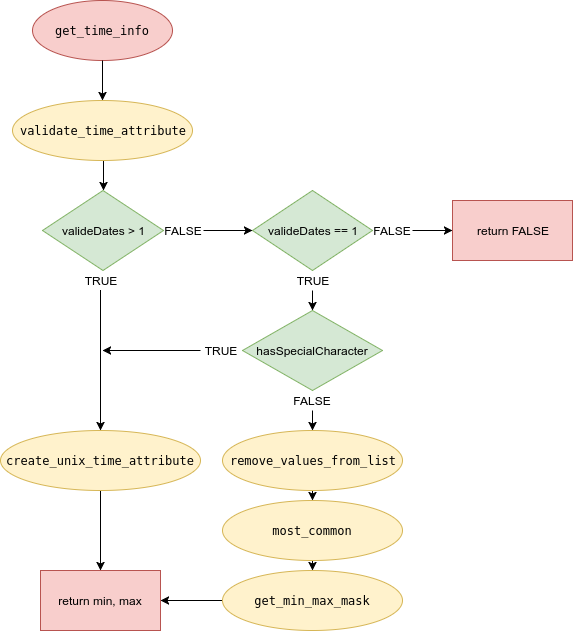
\includegraphics[width=0.8\textwidth]{../img/getTimeInfo.png}
\caption{Vývojový diagram publikace časové vrstvy}
\label{fig:plugin-chart}
\end{figure}

Posledním krokem je poté pouze export zjištěných hodnot do metadatového
souboru. Každé časové vrstvě je vypsán časový formát pro zobrazení
časových hodnot na webovém klientu. Dále název časového atributu,
minimální a maximální hodnota časového atributu ve formátu \textit{UNIX
TIME} a další parametry, které budou popsány a vysvětleny dále. V
případě, že data jsou validní a obsahují pouze jeden časový formát
je vypsán tento formát. Pokud tomu tak není a je použit pomocný atribut
s hodnoty ve formátu \textit{UNIX TIME}, je vypsán jeho název.

\subsection{Metadatový soubor}
\label{sssec:metadata}

Metadatový soubor (viz. kapitola \ref{sssec:gisquick-komponenty}, část
\textit{Gisquick plugin}) je textový soubor, který vniká publikací
projektu Gisquick pluginem. Obsahuje množství informací, které jsou
nutné pro správnou konfiguraci straně webového klienta.

Pokud jsou vrstvy při publikaci označeny jako časové a jejich data jdou
validní, jsou do nich vepsány následující hodnoty:

\begin{itemize}
\item\textit{unix} - parametr unix nabývá hodnoty \textit{TRUE}
v případě, že byl vytvořen pomocný atribut s časovými
hodnoty ve formátu \textit{UNIX TIME}. Slouží webovému
klientu k určení zda-li má k filtrování časové vrstvy
(viz. kapitola \ref{sssec:time-filtration}) použít daný formát
\textit{input\textunderscore datetime\textunderscore mask}, nebo
\textit{UNIX TIME}.
\item\textit{original\textunderscore time\textunderscore attribute}
- zde je uložen název časového atributu. Parametr slouží k
určení atributu při filtrování časové vrstvy (viz. kapitola
\ref{sssec:time-filtration}).
\item\textit{output\textunderscore datetime\textunderscore mask}
- obsahuje formát časového řetězce, který si uživatel
zvolil v roletovém menu \textit{Date Mask} (viz. kapitola
\ref{sssec:plugin-ui}). Tento parametr definuje formát, kterým
jsou zobrazeny časové hodnoty na straně webového klienta.
\item\textit{time\textunderscore values} - jedná se o pole
obsahující minimální a maximální hodnotu časového
atributu ve formátu \textit{UNIX TIME}. Na základě těchto
hodnot je na webovém klientu inicializovaný časový
posuvník (viz. kapitoly \ref{sssec:one-layer-filtration},
\ref{sssec:multiple-layers-filtration}).
\item\textit{input\textunderscore datetime\textunderscore mask} - tento
parametr je vytvořen pouze pokud není nutné vytvářet pomocný
atribut (viz. kapitola \ref{sssec:plugin-functionality}). Parametr
obsahuje formát časového řetězce zvoleného časového
atributu. Díky tomuto parametru může být pro potřeby filtrování
časové vrstvy převedena hodnota učená na časovému posuvníku
do stejného časového formátu v jakém je uložena (viz. kapitola
\ref{sssec:time-filtration}).
\item\textit{time\textunderscore attribute} - parametr
je vytvořen pouze pokud je nutné vytvářet pomocný
atribut obsahující hodnoty ve formátu \textit{UNIX TIME} a
obsahuje název tohoto atributu. Parametr slouží stejně jako
\textit{original\textunderscore time\textunderscore attribute}
k specifikaci atributu při filtrování časové vrstvy.
\end{itemize}

\newpage
\bigskip
\noindent

Níže je zobrazena ukázka části metadatového souboru. Ta obsahuje dvě
časové vrstvy, kdy každá z nich má odlišné parametry. Pro kompaktnost
ukázky zde parametry, které se netýkají implementovaného rozšíření,
zobrazeny nejsou:

\begin{verbatim}
{
"unix": false,
"time_values": [
1309471200.0,
1507672800.0
],
"input_datetime_mask": "YYYY-MM-DD",
"output_datetime_mask": "YYYY-MM-DD",
"original_time_attribute": "platiod",
},
{
"time_attribute": "UTconvert",
"unix": true,
"time_values": [
1309471200,
1507672800
],
"output_datetime_mask": "HH:mm",
"original_time_attribute": "platiod1",
}
\end{verbatim}

\newpage
\section{Implementace nástroje do webového klienta}
Webový klient obsahuje hlavní část implementace rozšíření pro podporu
časoprostorových dat. Jedná se o jednoduchý nástroj, který umožňuje
filtrovat mapové prvky jednotlivých časových vrstev na základě jejich
časového atributu. Časový interval je možné nastavit pomoci posuvníku,
nebo přímo pomocí kalendáře a hodinového ciferníku. Nástroj na
webovém klientu umožňuje dále vytvářet jednoduché animace. Uživatel
má možnost zmíněnou filtraci mapových prvků provádět pro jednotlivé
vrstvy, nebo pro více vrstev současně.

\subsection{Uživatelské rozhraní}
\label{sssec:gisquick-client-ui}

\begin{figure}[h!]
\centering
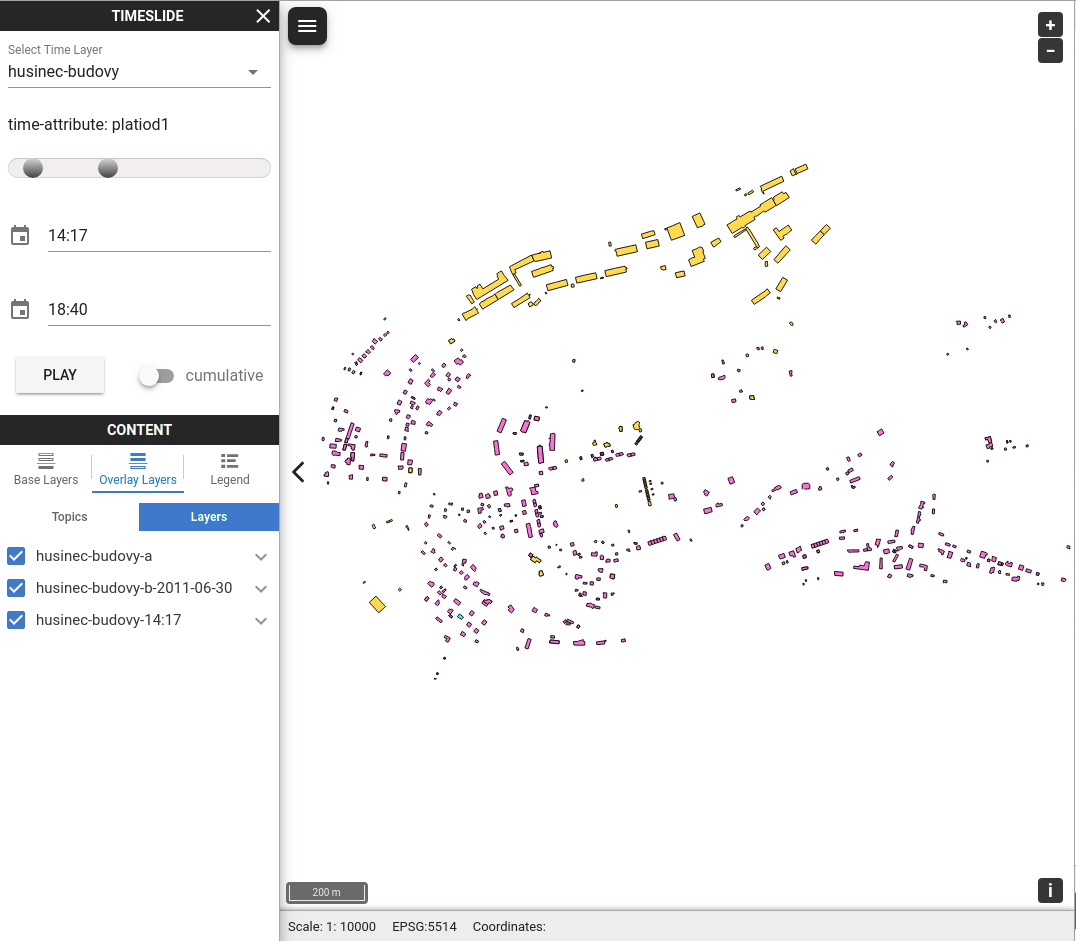
\includegraphics[width=1\textwidth]{../img/gisquick-time-tool.png}
\caption{Webové rozhraní Gisquick platformy s aktivovaným nástrojem
pro páci s časoprostorovými daty}
\label{fig:gisquick-client}
\end{figure}

Celý nástroj je ukrytý v postranním menu a obsahuje jen několik prvků,
které však uživateli poskytují velké množství operací. Všechny
jsou zobrazeny v obrázku \ref{fig:gisquick-client}. Od shora se jednotlivě
jedná o:

\begin{itemize}
\item\textit{roletové menu s výběrem časové vrstvy} - v
případě aktivace nástroje je toto pole jediný prvek, který
je uživateli zobrazen. Jako první krok je nejprve nutné vybrat
časovou vrstvu, která bude použita. Toho lze docílit pomocí
zmíněného roletového menu, které obsahuje všechny časové
vrstvy. Dále je zde možnost "All visible layers", která uživateli
umožňuje výběr všech viditelných časových vrstev.
\item\textit{jméno časového atributu} - tento prvek neumožňuje
uživateli jakoukoli interakci s nástrojem a má tedy čistě
informativní charakter. Je zde vypsán název časového atributu
vybrané vrstvy. Jeho existence je přínosná především v
případě, kdy projekt obsahuje více časových vrstev s odlišným
časovým parametrem. Při výběru možnosti "All visible layers" je
možné použít pouze vrstvy se stejným parametrem. Uživatel je tedy
tomto případě informován pro jaký parametr jsou vrstvy vybrány.
\item\textit{dvojitý časový posuvník} - jedná se posuvník
se dvěma
%%DT: nedokázal jsem přijít na lepší slovo, nez šoupátka
šoupátky. Díky němu je možné snadno a rychle mapové
prvky filtrovat. Uživatel tak ihned získá představu o jejich
rozmístění na časové ose. Minimum a maximum posuvníku odpovídá
minimu a maximu intervalu časových hodnot jednotlivé vrstvy. Pro
více vrstev se jedná o minimum a maximum sjednocení intervalů. Krok
je vždy určen jako jedna setina intervalu hodnot posuvníku.
\item\textit{časové štítky} - na dvou řádcích jsou dvě
textové pole s minimálním a maximálním datem filtrovaných
časových hodnot. Tato pole slouží k přesné definici
časového úseku. Každé z nich obsahuje integrovaný kalendář
s hodinovým ciferníkem pro určení hodnot. Časový formát
zobrazený v těchto polích je definován při publikaci projektu
(viz. kapitola \ref{sssec:plugin-ui}). Pokud formát neobsahuje
možnost zobrazení minut, nebo hodin, v tom případě se hodinový
ciferník nenabízí. Stejným způsobem není nabídnuta možnost
filtrování za pomoci kalendáře v případě, že časový formát
obsahuje jen hodiny, nebo minuty.
\item\textit{animační tlačítko s přepínačem} - tlačítkem \textit{PLAY}
je možné spustit animování aktivní časové vrstvy.  Ve chvíli, kdy je animace aktivována, změní se tlačítko na \textit{STOP}. Tím je možné animování zastavit. V implicitním stavu, kdy je spínač \textit{cumulative} vypnutý, jsou obě šoupátka posouvána současně. V případě jeho aktivace je vždy po jedné sekundě zvyšována hodnota horního šoupátka až do chvíle kdy dosáhne maxima posuvníku. V tom případě je zvyšována hodnota spodního šoupátka (viz. kapitola \ref{sssec:animation}).
\end{itemize}

\subsection{Princip časové filtrace}
\label{sssec:time-filtration}

Jak bylo zmíněno v kapitole \ref{sssec:qgis-server}, QGIS server nepodporuje ve specifikaci WMS operace \textit{GetMap} parametr \textit{TIME}. Z toho důvodu je nutné
použít obdobnou metodu, kterou používá MapServer, a to nahrazení
parametru \textit{TIME} parametrem \textit{FILTER}.

\noindent
Parametr \textit{FILTER} lze použít v operaci \textit{GetMap} následovně
\cite{qgis-service}:
\begin{verbatim}
http://myserver.com/?
REQUEST=GetMap
&LAYERS=mylayer1,mylayer2
&FILTER=mylayer1:"OBJECTID" = 3;mylayer2:'text' = 'something'&....
\end{verbatim}

Tato skutečnost dovoluje filtrovat časové vrstvy na základě jejich
časového atributu resp. jeho názvu a hodnoty. Lze tak filtrovat jednu
i více vrstev najednou. Za použití speciálních znaků jako jsou
\textit{‘AND’, ’OR’, ’IN’, ’=’, ’<’, ’>=’,  ‘>’,
’>=’, ’!=*,’(‘,’)’} lze rovněž filtrovat intervaly hodnot
a jejich sjednocení \cite{qgis-service}.

V implementovaném nástroji pro časovou filtraci je při filtrování použit
dvojitý časový posuvník. Proto je obsah parametru \textit{FILTER} vždy
tvořen jako textový řetězec, který v obecné formě vypadá následovně:

\begin{verbatim}
mylayer1:
"timeAttribute" >= 'lowerValue'
AND
"timeAttribute" <= 'upperValue'
\end{verbatim}

Parametr \textit{FILTER} podporuje hodnoty časového atributu v datovém
typu textového řetězce, nebo jako celé číslo. Pro zachování
konzistence výsledků filtrování je nutné, aby časový formát hodnoty
vstupující do parametru \textit{FILTER} korespondovaly s příslušným
formátem časového atributu. Z toho důvodu je při publikaci projektu
ve speciálních případech nutné vytvoření pomocného atributu
(\ref{sssec:plugin-functionality}). Ten obsahuje hodnoty časového atributu
převedeny do formátu \textit{UNIX TIME}. To dovoluje k časovým hodnotám
přistupovat jako k celým číslům. V případě časového filtrování
této vrstvy není tedy použit námi zvolený časový atribut, ale nově
vytvořený.

\subsection{Inicializace nástroje}
\label{sssec:initialization}

Pokud není volba \textit{Use cache} při publikování projektu vypnutá
(viz. obrázek \ref{fig:gisquick-plugin-layers}), používá Gisquick webový
klient pro zobrazování mapových vrstev předem vytvořených mapových
dlaždic uložených v mezipaměti serveru (viz. specifikace WMTS kapitoly \ref{sssec:ogc}). Pro možnosti filtrace vrstev
na základě jejich časové hodnoty parametru však tento způsob nelze
aplikovat. Bylo by totiž nutné vytvořit mapové dlaždice pro všechny
možné časové intervaly a kombinace vrstev. Z toho důvodu je při aktivaci
nástroje pro práci s časoprostorovými daty použit \textit{Lifecycle Hook
Created}. Jedná se o funkci, která se spustí jakmile je Vue komponent
inicializován. V ní je původní instance třídy \textit{ImageLayer}
uložena do proměnné \textit{originalLayer} a skryta. Následně je
vytvořena instance nová, která obsahuje stejné mapové vrstvy jako
původní. Ta je poté nastavena jako aktivní. V případě, že mapový obraz má být aktualizován, je nutné vždy specifikací WMS (viz. kapitola \ref{sssec:ogc}) znovu generovat jeho obsah. Pokud je nástroj vypnut
je použita původní instance a webový klient je tedy opět v původním
nastavení.

\subsection{Filtrace jedné časové vrstvy}
\label{sssec:one-layer-filtration}

První a také jediný krok, který lze po inicializaci časového nástroje
udělat je volba časové vrstvy. Zde je možno zvolit jednotlivé časové
vrstvy, nebo filtraci všech viditelných časových vrstev. Pokud je
vybrána možnost filtrace mapových prvků pouze jedné vrstvy, je tato
vrstva v případě jejího skrytí znovu zviditelněna. Následný postup
je popsán dále.

\bigskip
\noindent \textbf{Inicializace}

Nejprve nutná inicializace časového posuvníku. Na něm jsou závislé
další uživatelské prvky jako například \textit{časové štítky}
(viz. kapitola \ref{sssec:gisquick-client-ui}). Jeho minimální a maximální
hodnota je získána z metadatového parametru \textit{time\textunderscore
attribute} (viz. kapitola \ref{sssec:metadata}). Velikost kroku posuvníku
určena jako setina rozdílu jeho maximální a minimální hodnoty. Metoda
\verb|setSliderValue| inicializuje hodnoty šoupátek na jejich poslední
použité. V případě, že nebyla vrstva ještě filtrována, je hodnota
levého šoupátka rovna minimu časového posuvníku a hodnota pravého
šoupátka o krok časového posuvníku větší.

Stejně jako hodnoty parametru \textit{time\textunderscore attribute},
tak hodnoty šoupátek jsou v časovém formátu \textit{UNIX Time}, tedy
jako celočíselný datový typ. \textit{Vue.js} umožňuje nastavení
\textit{Watched Property}. Takto jsou nastavené proměnné hodnoty
šoupátek. Pokud se tedy jedna z hodnot změní je spuštěna metoda,
která provede převod původního celočíselného časového formátu
\textit{UNIX Time} do časového formátu \textit{output\textunderscore
datetime\textunderscore mask} zvoleného během publikace projektu
(viz. kapitola \ref{sssec:plugin-ui}, \ref{sssec:metadata}). Jakmile je tedy
časový posuvník inicializován, jsou ihned inicializovány i časové
štítky hodnotou v daném časovém formátu.

\bigskip
\noindent \textbf{Filtrace}
%\ref{appendix}
Způsob, jakým je aktualizována mapa na základě změny časových hodnot je
popsána v dokumentaci časového nástroje. Zde je popsán princip, kterým je
mapový obraz dle stávajícího nastavení časového nástroje aktualizován.

Při spuštění časové filtrace je v metodě \verb|updateSingleLayer|
provedeno několik po sobě jdoucích operací:
\begin{itemize}
\item\textit{detekce předem filtrovaných vrstev} - nejprve je
nutné zjistit, zda-li ostatní viditelné časové vrstvy již
filtrovány byly. V takovém případě je potřeba do parametru
\textit{FILTER} zahrnout nastavení předem filtrovaných
vrstev. Pokud by tak nebylo provedeno, z těchto časových
vrstev by byly zobrazeny všechny jejich mapové prvky. To
je provedeno metodou \verb|getFilterFromLayers|, která vrací
textový řetězec obsahující obsah parametru \textit{FILTER}
(viz. kapitola \ref{sssec:time-filtration}) časových vrstev,
které byly již předem filtrovány.
\item\textit{sestavení filtru pro danou vrstvu} - další krok
zahrnuje vytvoření obsahu parametru \textit{FILTER} pro právě
filtrovanou vrstvu. Tento krok se liší v závislosti na existenci
pomocného časového atributu s hodnoty ve formátu \textit{UNIX
TIME} (viz. kapitola \ref{sssec:plugin-functionality}). Parametr
\textit{unix} v metadatovém souboru (viz. kapitola
\ref{sssec:metadata}) obsahuje informaci o jeho vytvoření.
\begin{itemize}
\item\textit{unix = TRUE} - znamená to, že filtrace není
provedena nad hodnoty původního časového atributu, ale
pomocného atributu. Pro tuto kofiguraci je textový řetězec
sestaven pouze z parametrů poskytovaných metadatovým
souborem. Pro časovou hodnotu je přímo použita hodnota
posuvníku, která je v časovém formátu \textit{UNIX TIME}.
\item\textit{unix = FALSE} - v tomto případě je
nutné nejprve časové hodnoty převést z formátu
\textit{UNIX TIME} do textového řetězce, který
svým časovým formátem odpovídá formátu časového
atributu dané vrstvy. Formát pro záznamy časového
atributu je součástí metadatového souboru jako
\textit{input\textunderscore datetime\textunderscore mask}
(viz. kapitola \ref{sssec:metadata}). Sestavení textového
řetězce je poté obdobné jako v předchozím případě.
\end{itemize}
Na konci tohoto kroku jsou poté spojeny dohromady obsahy parametru
\textit{FILTER} z ostatních časových vrstev a nově vytvořený.
\item\textit{nastavení filtrované vrstvy} - tento krok je nezbytný
z několika důvodů. Je nutné uložit hodnoty časového posuvníku
v případě že vrstva bude v budoucnu filtrována znovu. Dále je
nutné uložit použitý obsah parametru \textit{FILTER}, který
je použit při filtrování ostatních časových vrstev. Jako
poslední věc je změněn název vrstvy tak, aby obsahoval její
jméno spolu s časovou hodnotou. Tímto způsobem uživatel ihned
ví, které vrstvy byly již filtrovány.
\item\textit{provedení operace GetMap} - v posledním kroku je
metodou \verb|updateParams| poslán požadavek na server obsahující
parametr \textit{FILTER} s obsahem složeným z filtru pro všechny
viditelné časové vrstvy. Server vrátí v odpovědi mapový obraz s
filtrovanými mapovými prvky, pomocí kterých je původní mapový
obraz nahrazen.
\end{itemize}

\begin{figure}[h!]
\centering
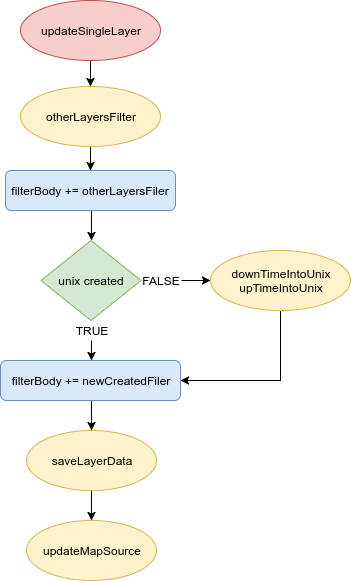
\includegraphics[width=0.5\textwidth]{../img/getSingleLayer.png}
\caption{Vývojový diagram filtrace více časových vrstev najednou}
\label{fig:single-chart}
\end{figure}

\subsection{Filtrace všech viditelných časových vrstev}
\label{sssec:multiple-layers-filtration}

Možnost selekce více vrstev je možné aktivovat v roletovém menu
obsahujícím jednotlivé časové vrstvy. Výběrem \textit{Select all
visible layers} je umožněno provádět filtraci mapových prvků pro
všechny viditelné časové vrstvy najednou.

\bigskip
\noindent \textbf{Inicializace}

Jednotlivé časové vrstvy mohou obsahovat navzájem odlišné
časové atributy, které v jistých případech nedovolují společnou
filtraci. Například pokud by projekt obsahoval dvě odlišné časové
vrstvy, kdy jedna by zachycovala časový průběh v intervalu jednoho dne
a druhá v intervalu jednoho roku. Výsledný krok časového posuvníku by
v takovém případě nebyl schopný postihnout nekonzistentní rozdělení
mapových prvků na časové ose. Z toho důvodu je při výběru možnosti
\textit{Select all visible layers} nejprve zjištěno, zda-li všechny
viditelné časové vrstvy mají zvoleny stejný, nebo odlišný časový
atribut. Tato zkutečnost je zjištěna metodou \verb|checkMultipleAttributes|,
která pro všechny viditelné časové vrstvy zjistí unikátní časové
atributy a uloží je do pole. Pokud takové pole obsahuje více, než jeden
prvek je zobrazeno další roletové menu ve kterém je nutné časový
atribut specifikovat.

Při inicializaci časového posuvníku je nutné brát v potaz
odlišné časové intervaly jednotlivých časových vrstev. Metoda
\verb|getSliderRange| postupně projde všechny viditelné
časové vrstvy mající zvolený časový atribut a z hodnot jejich
\textit{time\textunderscore values} (viz kapitola \ref{sssec:metadata}) určí
celkové maximální a minimální hodnoty. Tímto způsobem je zajištěno,
že všechny hodnoty časového atributu pro všechny časové vrstvy budou
náležet intervalu daného minimální a maximální hodnotou časového
posuvníku. Hodnoty šoupátek jsou nastaveny na minimální hodnoty
intervalu časového posuvníku, resp. na hodnotu, která je o časový
krok větší. Není přitom zohledňováno předchozí použití časových
vrstev při jejich filtraci tak, tako je tomu u fitrace jednotlivých vrstev.

Dále je nutné zajistit, aby časové hodnoty zobrazované na webovém
klientu, při filtraci více vrstev najednou, měly společný časový
formát. Časový formát je pro jednotlivé vrstvy definovaný v metadatovém
souboru (viz kapitola \ref{sssec:metadata}). Metoda \verb|setDateMask|
má za úkol mezi časovými formáty filtrovaných vrstev najít takový,
který poskytuje nejdetailnější zobrazení. Pokud tedy jedna z vrstev
má nastaveno zobrazování s podrobností minut, je její časový
formát upřednostněn. Metoda pro jednotlivé časové formáty nejprve
zjišťuje zda-li obsahují zároveň roky, hodiny a minuty. Pokud ano je
první nalezený formát použit. Pokud tomu tak není je hledán formát
obsahující alespoň roky. V případě, že ani takový není nalezen,
je použit časový formát první časové vrstvy.

Pro správné zobrazení kalendáře, hodinového ciferníků a
pro výběr hodnot časových štítků je nutné zjistit, jestli
nalezený časový formát obsahuje datum a čas. K tomu slouží metoda
\verb|maskIncludeDate|. Na základě jejího výsledku je skryta možnost
výběru časových hodnot pomocí kalendáře. Zobrazení hodinového
ciferníku je řešeno obdobně s tím rozdílem, že k detekci času v
časovém formátu je použito JavaScriptové metody \verb|includes|. Tato
metodika je provedena jak při výběru více časových vrstev, tak při
výběru jednotlivé vrstvy.

\bigskip
\noindent \textbf{Filtrace}

Princip a jednotlivé kroky samotné filtrace mapových prvků pro všechny
zobrazené časové vrstvy odpovídají popsanému principu pro filtraci
jednotlivých vrstev. Je zde však jedna podstatná změna při vytváření
obsahu parametru \textit{FILTER}. V metodě \verb|updateMultipleLayers| je
oproti metodě \verb|updateSingleLayer| přidán cyklus, který prochází
jednotlivě všechny viditelné časové vrstvy a zjišťuje jestli jejich
časový atribut je shodný s časovým atributem filtrovaných časových
vrstev. Dále je sestaven obsah parametru \textit{FILTER}. Pro každou vrstvu
mohou nastat dva případy:
\begin{itemize}
\item\textit{atribut není totožný} - pokud již byla
vrstva předem filtrována obsahuje použitý obsah parametru
\textit{FILTER}. Ten je v tomto případě zjištěn a
přidán do nově vytvářeného obsahu.
\item\textit{atribut je totožný} - časová vrstva je
filtrována a je tedy nutné sestavit obsah parametru
znovu. Tento princip je stejný jako v případě filtrace
jednotlivé vrstvy. Obsah parametru je rovněž přidán do
nově vytvářeného obsahu. Pro vrstvu jsou navíc uloženy
stejné hodnoty jako v případě filtrace jednotlivých
vrstev. Pokud by tedy vrstva byla znovu samostatně
filtrována, inicializuje se časový posuvník naposledy
uloženými hodnoty.
\end{itemize}
Pokud jsou všechny viditelné časové vrstvy zpracovány je nově vytvořený
obsah parametru \textit{FILTER} použit při operaci \textit{GetMap} stejným
způsoben jako u filtrace jednotlivé vrstvy.

\begin{figure}[h!]
\centering
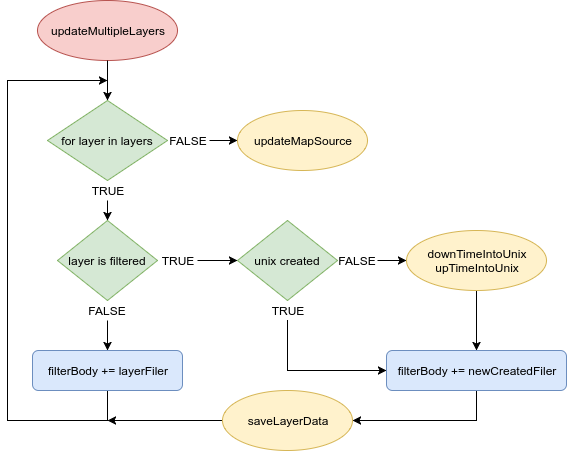
\includegraphics[width=0.9\textwidth]{../img/getMultipleLayers.png}
\caption{Vývojový diagram filtrace více časových vrstev najednou}
\label{fig:multiple-chart}
\end{figure}

\subsection{Animace filtrace}
\label{sssec:animation}

Jak pro jednotlivé vrstvy, tak pro více vrstev najednou je možnost
provádět filtraci mapových prvků automatizovaně a vytvářet tak
jednoduché animace. K tomu slouží tlačítko \textit{PLAY} na spodní
straně nástroje viz. kapitola \ref{sssec:gisquick-client-ui}.

Jedná se o jednoduchou metodu \verb|animate|, která s prodlevou jedna
sekunda mění hodnotu časového posuvníku. Tato metoda pouze kontroluje
hodnotu proměnné \textit{animateStop}. Pokud je tato hodnota FALSE, je
volána metoda \verb|newFrame|. Metoda \verb|newFrame| při každém svém
zavolání zkontroluje hodnotu spínače \textit{cumulative}:
\begin{itemize}
\item\textit{cumulative = TRUE} - pokud je hodnota horního šoupátka
menší než maximální hodnota časového posuvníku, je zvýšena
o velikost kroku posuvníku. Pokud je hodnota horního šoupátka vyšší a rozdíl obou šoupátek je větší, než velikost kroku posuvníku, je zvýšena hodnota spodního šoupátka.
\item\textit{cumulative = FALSE} - pokud je hodnota horního šoupátka
menší než maximální hodnota časového posuvníku, jsou zvýšeny
společně obě hodnoty šoupátek o krok časového posuvníku.
\end{itemize}
Po zvýšení hodnot je zavolána metoda \verb|getNewUrl| (viz. kapitola
\ref{sssec:one-layer-filtration}), která aktualizuje mapový obsah podle
nově nastavených filtrovaných hodnot. Nakonec v případě, že hodnota
\textit{animateStop = FALSE}, zavolá metoda \verb|newFrame| rekurzivně sama sebe s časovou prodlevou jedna sekunda.

\begin{figure}[h!]
\centering
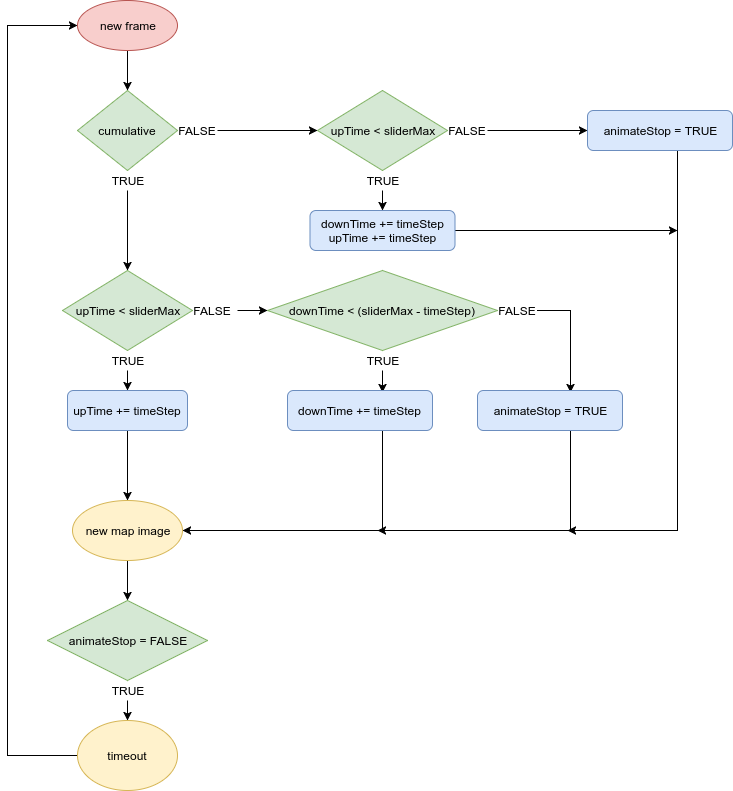
\includegraphics[width=0.9\textwidth]{../img/animate.png}
\caption{Vývojový diagram metody animate}
\label{fig:animate-chart}
\end{figure}
